\chapter{Background}
\label{ch:background}
\acresetall

This chapter aims to give the reader the necessary background to ad hoc routing,
attacks on ad hoc networks, and about the proxy certificates concept in order to
understand the concepts and discussions of this thesis.

\section{Mobile Ad Hoc Network}
An ad hoc network is a network of nodes which communicate with each other and
through each other, i.e. nodes act as both regular end nodes and as intermediate
nodes, similar to routers in regular networks. Because nodes in an ad hoc
network can route packets from one node to another until its destination, ad hoc
networks do not need an infrastructure with routers such as regular networks
do \cite{perkins2008ad}. Without an infrastructure ad hoc networks can be
established spontaneously and with no, or minimum, pre-configuration depending
on the implementation in use.

\begin{figure}[h]
	\centering
	\subfloat[Infrastructure Mode]{\label{fig:infrastructure_mode}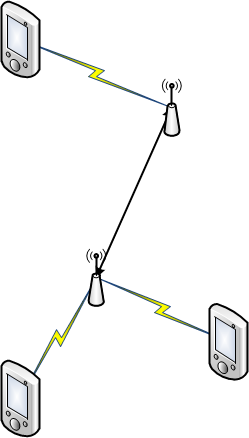
\includegraphics[width=0.3\textwidth]{images/background_net_infrastucture.png} }
	\hspace{15mm}
	\subfloat[Ad Hoc Mode]{\label{fig:adhoc_mode}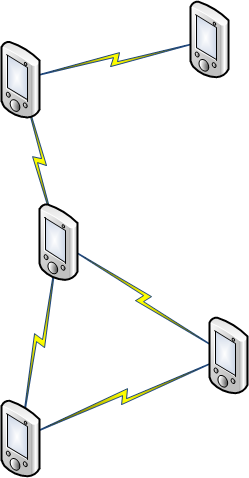
\includegraphics[width=0.3\textwidth]{images/background_net_adhoc.png}} 
	\caption{Difference between a regular infrastructure network and an ad hoc network}
	\label{fig:background_networks}
\end{figure}

Figure \ref{fig:background_networks} depicts the difference between a regular
wireless network and an ad hoc network. In \ref{fig:infrastructure_mode} there
are three mobile nodes connected to each other through two wireless access points
(infrastructure), while in \ref{fig:adhoc_mode} there are five nodes connected
to each other and through each other. In infrastructure mode an end node only
accepts packets addressed to itself, while in ad hoc mode the node will try to
forward packets addressed to other nodes (on the network layer). They will
however not accept packets sent to other link-layer addresses.

A \ac{MANET} is a subset of ad hoc networks, in which nodes are specified as
non-stationary wireless nodes, i.e. a \ac{MANET} consists of several mobile
nodes communicating with each other, and through each other even while on the
move. With \acp{MANET} nodes are always on the move and must therefore update
their routing tables continously to make sure full paths between nodes are
updated as quickly as possible, i.e. a minimal routing path convergence is
necessary.

In this thesis the terms ``network'', ``\ac{MANET}'', and ``ad hoc network''
are used interchangeably meaning a ``\ac{MANET}'' as described in this section
unless otherwise specified.

\subsection{Routing}
There are many routing protocols for ad hoc networks and some of the popular
protocols are OLSR \cite{olsr_paper}, B.A.T.M.A.N. \cite{batman_rfc}, Babel
\cite{rfc6126}, DSDV \cite{he2002destination}, and AODV
\cite{Perkins:2003:AHO:RFC3561} which all fall into one of the two main
categories of ad hoc routing - i.e. ``reactive'' and ``pro-active'' routing
protocols. In this thesis a pro active routing protocol is used in the system
design, and as such an introduction to this type of protocol is necessary.

\subsubsection*{Pro-active Routing Protocols}
As the name suggests, a pro active routing protocol finds or creates routing
paths before, i.e. pro actively, the paths are requested. Essentially this means
that the routing protocol on a node has to regularly share routing information
with other nodes it can communicate with. This can be done in a huge variety of
ways - from storing full paths to all known nodes and broadcast this information
to all nodes regularly, to only storing a first hop in the direction of the
known nodes, and only telling your neighbors that you have a route to some other
node instead of the full route.

Each method might have some advantages over the other, i.e. storing full paths
and sending all this information to all nodes in the network might minimize the
chances of routing loops and route flappings, but this method would have a huge
overhead in signalling traffic. The latter method would have much less overhead,
but it is more difficult to avoid routing loops and/or route flapping.

\subsubsection*{Reactive Routing Protocols}
In opposition to pro-active protocols, reacive protocols calculates and updates
routes when they are needed, i.e. when data is being sent. The advantages of
this strategy is conserving power used in obsolete/non-necessary routing
calculations, but the downside being that the protocol might react more slowly
to topology changes.

\subsection{Challenges}
There are a multitude of challenges to solve in regards to ad hoc networking,
and especially so in modbile ad hoc networking. First there are challenges
regarding routing such as route flapping and routing loops, then there is the
issue of power conservation as modile ad hoc nodes usually runs on battery
power, and last, but definately not least, there is the issue of security.

\subsubsection*{Route Flapping}
Route flapping is a term describing rapid route changes when there are multiple
possible routes between two nodes. Sometimes two routes might be almost equally
good and might stay that way for a while, which might lead routes in a node's
routing table to constantly change between the two. In such scenarios a routing
protocol might solve the problem by not changing routes unless the other route
is a significantly better route, or if it has been slightly better for a longer
period of time. Which is the better solution is difficult to determine and is
one of many reasons why there are a huge amount of contesting ad hoc routing
protocols, and this question remains unresolved.

\subsubsection*{Routing Loops}
You have a routing loop if a path between two nodes passes through one or more
node(s) on the route more than once. When nodes have wrong, incomplete, or just
different routing information from one another then two nodes in the network
might choose to route the same packets through different paths, which might
lead the route to eventually return to nodes which have already received and
forwarded said packets.

In a \ac{MANET} where routes might change very often, the chances of two nodes
having different routing information is high. Routing loops can therefore become
a severe problem in \acp{MANET}, suggesting implementations should use a
protocol that has some mechanisms to minimize the chances of routing loops,
and/or detecting routing loops and removing them after the fact.

\subsubsection*{Power Conservation}
With mobile nodes in a \ac{MANET} power consumption can become a huge hindrance.
Because pro active routing protocols sends routing information regularly, even
if they are not needed, they might be wasting energy compared to reactive
protocols that only calculates routing paths when application data is sent
through the network.

This issue will also be very much affected by the security implementation on top
of the ad hoc routing protocol. If. for example, every packet is to be digitally
signed, a hashing operation and an public key encryption operation would be
performed on each packet - using a lot of energy. When designing the
authentication solution this issue needs to be addressed.

\subsubsection*{Security}
Security can be divided in multiple fields of interest such as (but not limited
to) \textit{confidentiality}, \textit{integrity}, \textit{authenticity}, and
\textit{access control} to name a few. Whatever the security feature is, it
usually depends on \emph{authentication}.

Acheiving a secure initial authentication is a very difficult task even in
regular networks, but using a verifyable identity based upon this initial
authentication is conquered using \acp{PKI}. In a \ac{MANET}, possibly without
Internet access, this task is again very difficult. Therefore, one ends
up with the original problem - doing initial authentication all over again. As this
is topic is greatly discussed throughout the thesis there is no point in
elaborating more at this point.

\section{B.A.T.M.A.N.}
BATMAN \cite{batman_rfc} is an increasingly popular routing protocol for
wireless ad hoc networks, as seen by the fact its taken into the Linux kernel
net tree\footnote{\url{http://www.open-mesh.org/wiki/open-mesh/2011-03-17-batman-adv-and-the-penguin}}.
The name is an abbreviation for ``Better Approach To Mobile Ad hoc
Networking''. The motivation behind developing BATMAN was to replace the
Optimized Link State Routing Protocol (OLSR) \cite{why-starting-batman} because
of the inherent difficulties that protocol has, as explained below.

\subsection{From OLSR to BATMAN}
OLSR is a pro-active routing protocol, which means that participating nodes
regularly exchange routing information with each other. According to the BATMAN
developers the problem with OLSR is that every node in the network calculates
the whole routing path, which is a complex way to do it. Not only is it
difficult to make sure all nodes have the same information at the same time,
it also needs (relatively) much storage and computation time. If nodes sit on
different routing information this concept leads to routing loops and heavy
route flapping. The result is many patches to the protocol that defies the
protocol standard in order to make it more suitable \cite{why-starting-batman}.

The BATMAN developers therefore wanted to start with a clean slate. They decided
amongst other things that each node should only know the next hop, i.e. the
link-local neighbor that is the path between itself and the destination. In
many ways, what they did was to make a simpler and easier to understand
protocol. For instance, the way BATMAN calculates the optimal route, i.e. the
next jump, is by comparing the number of routing messages it has received from
each node and who was the last sender.

\subsection{BATMAN Protocol Explanation}
The routing messages sent in BATMAN are called \acp{OGM}. Figure
\ref{fig:original_ogm} shows the packet format with all header fields. The
\ac{OGM} format has changed since the draft specification was published
\cite{batman_rfc}, but there is no official publication with the new packet
format as of yet. The updated packet format can be found in the project's
internal documentation\footnote{\url{http://gitorious.org/batman-adv-doc/}}.
The packet format found in the draft specification belong to the older version
III of the BATMAN algorithm. The algorithm used in this thesis is version IV.

\begin{figure}[h]
	\centering
  	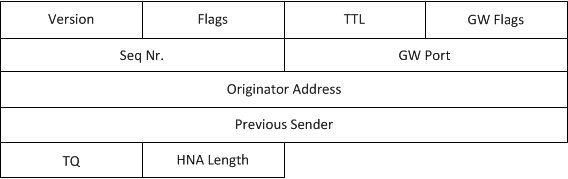
\includegraphics[width=\textwidth]{images/original_ogm.png}
  	\caption{BATMAN's \acf{OGM} packet format.}
	\label{fig:original_ogm}
\end{figure}

The real workhorse of the packet is the ``Originator Address'' field which
carries the host address of the node 'A' that broadcasted the \ac{OGM}. When a
node 'B' receives this message it checks if the originator address and source
address of the IP header are the same - if so the two nodes are direct
neighbors. B then forwards the \ac{OGM} only changing the ``\ac{TTL}'' and
``Previous Sender'' fields. B's neighbors who receive this OGM from A through
B also forwards the packet and so on. All \acp{OGM} inside the BATMAN network
are broadcasted and rebroadcasted until the TTL has dropped to zero, or until
the nodes receive an \ac{OGM} they have previously sent themselves.

This way all \acp{OGM} will be received and rebroadcasted by all nodes in the
network and all nodes will learn the existence of each other and which nodes are
the first hop between them and the other nodes, i.e. the first hop of the path.
All nodes and their first hops in their paths are stored in a list called an
``Originator List''.

\begin{figure}[ht!]
	\centering
	\subfloat[TTL = 50]{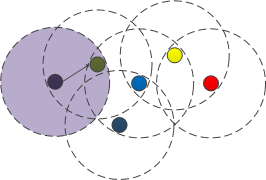
\includegraphics[width=0.4\textwidth]{images/ogm_packet_flow_1.png}}
	\hspace{10mm}
	\subfloat[TTL = 49]{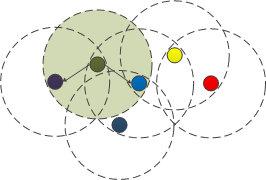
\includegraphics[width=0.4\textwidth]{images/ogm_packet_flow_2.png}}
	\\ 
	\subfloat[TTL = 48]{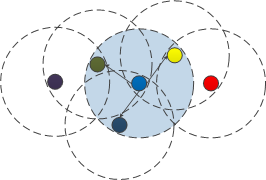
\includegraphics[width=0.4\textwidth]{images/ogm_packet_flow_3.png}}
	\hspace{10mm}
	\subfloat[TTL = 47]{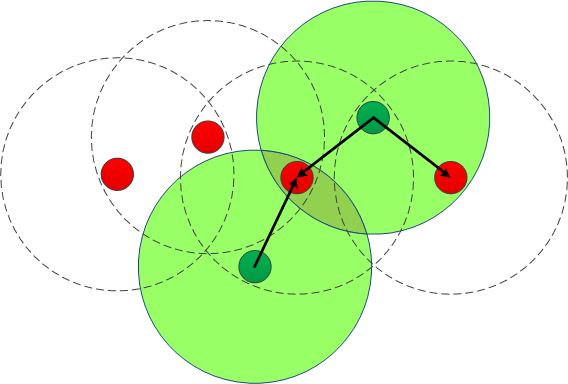
\includegraphics[width=0.4\textwidth]{images/ogm_packet_flow_4.png}}
	\\ 
	\subfloat[TTL = 46]{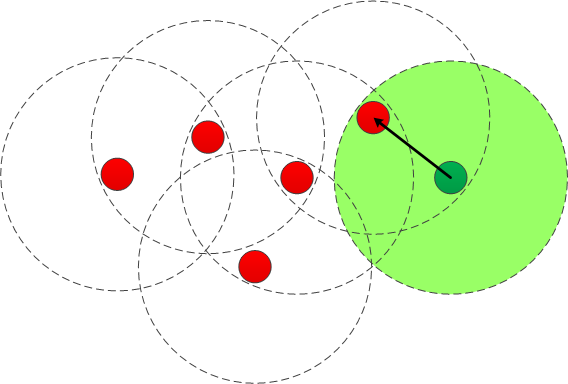
\includegraphics[width=0.4\textwidth]{images/ogm_packet_flow_5.png}}
	\caption{Flow of one OGM originating from the left-most node.}
	\label{fig:ogm_packet_flow}
\end{figure}

Figure \ref{fig:ogm_packet_flow} shows how an \ac{OGM} is broadcasted and
forwarded throughout the network. The packet originates from the left-most node,
and for each node that receives the packet, they forward it to their neighbors
again.

When a node which has already received and forwarded an \ac{OGM} receives the
same \ac{OGM} from another node at a later point - it drops that packet so the
network will not get flooded by forwarding the same \acp{OGM} until its \ac{TTL}
is zero. This is also necessary in order to prevent routing loops. BATMAN uses
sliding windows to detect whether an \ac{OGM} has been received before or not.

\subsection{BATMAN Daemon vs. BATMAN Advanced}
There are two completely different versions of the BATMAN ad hoc routing
protocol\footnote{\url{http://www.open-mesh.org/wiki/open-mesh/BranchesExplained}},
and the one described so far has been the BATMAN Daemon, or \emph{batmand}. This
version has the benefits of being a network layer protocol making the
authentication scheme proposed in this thesis sound. However, there is a new
version called BATMAN Advanced, or \emph{batman-adv}, which operates on the
link layer instead. This version breaks the standard layering principle as it
routes packets throughout the network on the link layer, encapsulating
everything above such as IP and DHCP packets. Because of this huge difference
the design proposed in this thesis will not work with batman-adv, at least not
without major changes to the design. Note therefore that whenever BATMAN is
mentioned in this thesis, it is the BATMAN Daemon (version 0.3.2) which is
being referred to.

\section{Proxy Certificates}
\label{sect:pc}
A \acf{PC} is a X.509 Certificate ``(\ldots) derived from, and signed by, a
normal X.509 Public Key End Entity Certificate or by another Proxy Certificate
for the purpose of providing restricted proxying and delegation within a PKI
based authentication system.'' \cite{rfc3820}.

The idea behind \acp{PC} was to overcome challenges with authentication
using e.g. \ac{SSO} in a Grid Computing setting \cite{foster1998security}. Here
a user might want to initiate a process that runs over several entities in the
grid, and maybe even after the user has logged off. Therefore a way to delegate
the user's rights to the entities running the processes for him was necessary.

Simply understood, a \ac{PC} is a public key certificate signed not
by an \ac{CA}, but by an \ac{EEC} or another \ac{PC}. With such certificates one
can delegate rights on behalf of one self, i.e. if you issue a \ac{PC} to some
other entity, that entity will be able to act on your behalf. \acp{PC} allows
the use of restrictions, given in a proxyPolicy field. This way the issuer can
decide which of its own rights the issuee shall have, granted the issued \ac{PC}
cannot have more or elevated rights than the issuer of the \ac{PC}.

\section{Attacks on Mobile Ad Hoc Networks}
There are a multitude of attacks on mobile ad hoc networks
\cite{goyal2010literature}, and a lot of them are essentially \ac{DoS} attacks
such as jamming. However, in this thesis attacks on the routing model is of
more interest and below are two very different attacks on our routing model.

\subsection{Wormhole Attack}
A wormhole attack is an attack in which the attacker is able to set up a so
called \emph{wormhole} between two distant nodes in the network, and using this
wormhole to e.g. copy a packet (such as in a replay attack) and send it to a
receiver at the other end before the original packet arrives (preplay).

\begin{figure}[h]
	\centering
  	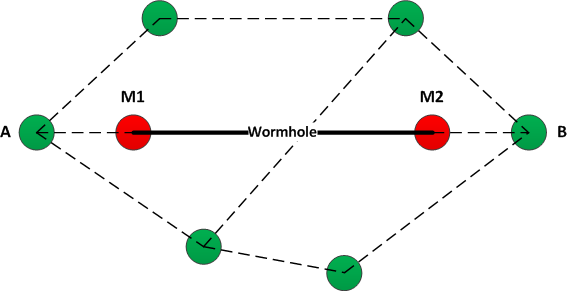
\includegraphics[width=\textwidth]{images/wormhole_attack.png}
  	\caption{Wormhole attack between node A and B.}
	\label{fig:wormhole_attack}
\end{figure}

Figure \ref{fig:wormhole_attack} shows the idea behind the wormhole attack. Here
we have a network of trusted nodes (green) and two malicious nodes (red). The
trusted nodes are communicating via wireless links, which the malicious nodes
are able to pick up. The wormhole between the two malicious nodes can be a fiber
channel, or it might just be a wireless radio link where the two malicious nodes
have much higher transmitting power than the trusted nodes, extending their
transmitting range.

The simplest attack using this model against an ad hoc routing protocol would be
for the first malicious node (M1) to copy a routing announcement from node A,
send it through the wormhole to M2, and have M2 forward the packet to node B
using both mac layer and network layer address spoofing. If successful, i.e.
this packet arrives before the re-broadcasts from the other slower nodes, it
would fool node B to believe that node A is a direct neighbor and he would
update his routing tables accordingly.

\subsection{Suppress Replay Attack}
A suppress replay attack, sometimes called a pre-play attack, is an attack in
which an attacker is able to intercept and suppress a packet, or parts of a
packet in air. For instance, if a packet appended with some secret is sent over
a radio link, the attacker might be able to jam the first part of the packet and
receive the secret. The original recipient would also just receive the secret
part, but would on the link layer drop the packet because there would be a
\ac{CRC} mismatch (or no \ac{CRC} at all).

At this point the attacker could be able to create a new falsified packet, and
append it with the secret - which the recipient might trust depending on the
authentication scheme used.

\section{Related Work}
There are many proposals of security designs for \acp{MANET}, and a very few
actual implementations based on some specific routing protocols. None of the
implementations found by this author would be applicable for the BATMAN
protocol, but some of the design proposals probably would.

Seno et al. propose a system design based on a distributed CA, using clustering
of nodes and an offline/out-of-band authentication scheme \cite{hosseinisecure}.

Another related authentication scheme is proposed by Dey and Datta which have a
more mathematical approach to the problem \cite{springerlink:Haimabati}. This
solution requires a predefined unique ID and special hardware with a hidden and
secure algorithm (i.e. smart card), and is probably better suited for a
military application than emergency situations.

Sanzgiri et al. proposed an authentication scheme for ad hoc routing called
Authenticated Routing for Ad hoc Networks (ARAN), by adding a signature
extension to the AODV reactive routing protocol \cite{sanzgiri2005authenticated}.

Additionally, some believe the computational costs using asymmetric keys for ad
hoc authentication is too great which lead to the Ariadne protocol
\cite{hu2005ariadne}, and the Secure Routing Protocol
\cite{papadimitratos2002secure}.

Nyre et al. published a design of an hierarchical authentication system for the
OLSR ad hoc routing protocol \cite{nyre2009secure}.

The problems with most of the related work are their complexity, high
computational costs and/or non-scalability when networks running implementations
based on their design grow large - and these things are what separates this
thesis from the other works.
